
To set the stage for what follows in this chapter, we first give a brief overview of some of the concepts in the \AF notation with the help of an example shown in \fig{af:1}.

The diagram illustrates the regulation of peroxisome proliferator-activated receptor delta (PPAR delta, a nuclear hormone receptor) on brown fat metabolism, a redraw from Fig 7E of Pan et. al~\cite{Pan:2009}.  The rectangle nodes represent \emph{biological activities} - activities from biological materials.  The type of material is indicated in the units of information decorating on the activity nodes (See \sect{af:biologicalActivity}).  Each biological activity can influence, or be influenced by, other biological activities, and such relationships are represented in \AF by lines with arrows and other decorations.  It should be noted that the essence of \AF is to show the flow of activities from one entity to another or within the same entity.  For example, in the diagram, it shows that PPAR$\delta$ positively influences the Twist-1 gene expression.  The underlying mechanisms of how the influence occurs may not be known and is not capture in the diagram.  If the mechanism is known, the details should be described in annotation or captured in other SBGN languages, such \PD and/or \ER.

\tab{component-summary} summarizes the different SBGN abstractions described in this chapter.

\newcolumntype{P}[1]{>{\raggedright\hspace{0pt}\arraybackslash}p{#1}}

\begin{table}[bh]
  \centering
  \small
  \begin{tabular}{@{}llP{2.4in}P{1.6in}@{}}
    \toprule
    \textbf{Component} & \textbf{Abbrev.} & \textbf{Role} & \textbf{Examples}\\
    \midrule
    Activity node
    & AN
    & A functional unit that can affect, or be affected by, another functional unit.
    & Biological activity \\[0.5em]

    Container node	
    & CN
    & An encapsulation of one or more other SBGN constructs
    & Compartments \\[1.6em]

    Modulating arc
    & MA
    & Links between different activities to indicate influences.
    & Positive influence, Negative influence \\[0.5em]
    
    Auxiliary units
    & AU
    & A decorating glyph to the AN to provide additional information of the node, such as the property where the activity is originated
    & Unit of information   \\[1.6em]
    
    Logical operators
    & ---
    & Combines one or several inputs into one output
    & Boolean \emph{and}, \emph{or}, \emph{not}, \emph{delay} \\
    \bottomrule
  \end{tabular}
  \caption{Summary of \AF components and their roles.}
  \label{tab:component-summary}
\end{table}

\begin{figure}[H]
\centering
\vspace*{-0.75em}
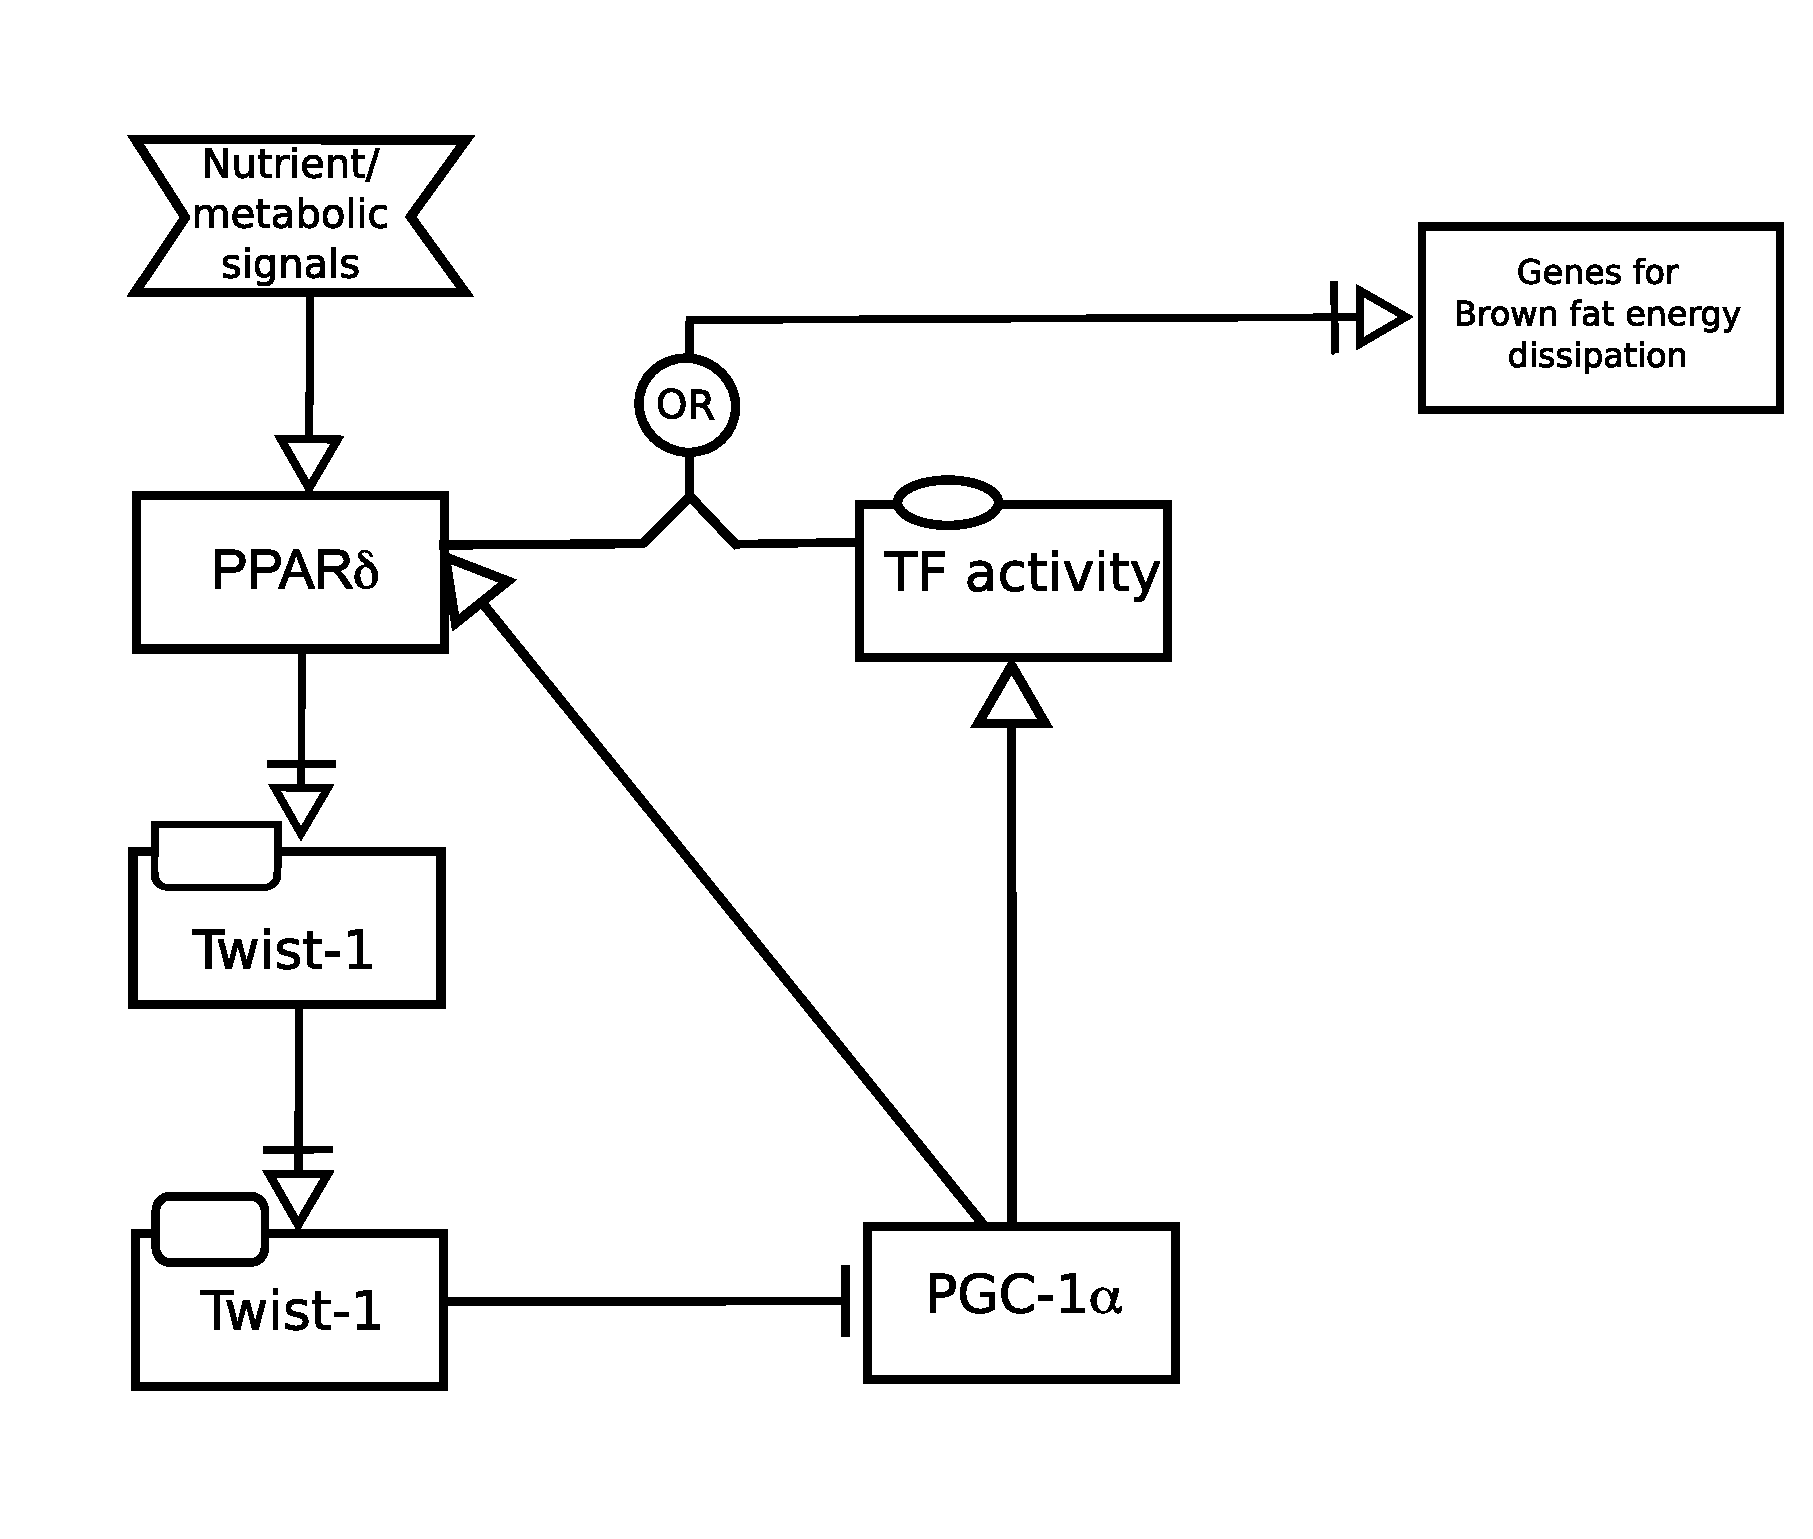
\includegraphics[scale=0.4]{examples/PPAR}
\caption{This example of \AF is based on Figure 7E of Pan el. al.~\cite{Pan:2009}.  It depicts the effect of nutrients and metabolic signals on brown fat metabolism through PPAR$\delta$. The signal, shown as a perturbation, positively influences the nuclear hormone receptor PPAR$\delta$, which in turn stimulates the Twist 1 gene expression.  Please note the different \emph{units of information} on Twist-1 activity nodes that indicate the activity from different biological materials (gene and protein). The Twist-1 protein negatively influences the PGC-1$\alpha$ activity, which positively influences PPAR$\delta$ and other unspecified transcription factor activity to stimulate the expression of genes for brown fat energy dissipation. Therefore, the Twist-1, induced by PPAR$\delta$, serves as a negative feedback regulator of PGC-1$\alpha$ in brown fat metabolism.}
\label{fig:af:1}
\end{figure}
